\documentclass[11pt]{beamer}
\usepackage[utf8]{inputenc}

\usetheme{Boadilla}
\usecolortheme{dolphin}
\usepackage{color,soul}
\usepackage{multicol}
\usepackage{multirow}
\usepackage{amsmath}
\usepackage{amsfonts}
\usepackage{amssymb}
\usepackage{algpseudocode} % uses algorithmicx package automatically
\usepackage{mathrsfs}
\usepackage{graphicx}
\usepackage{tikz}
\usetikzlibrary{calc}
\usetikzlibrary{shapes.geometric}
\usepackage{pgfplots}
\usepackage{subcaption}

\tikzstyle{trap}=[trapezium, draw, minimum width=12cm,trapezium left angle=120,trapezium right angle=60]

\begin{document}
\begin{frame}
  \begin{figure} 
    \centering
    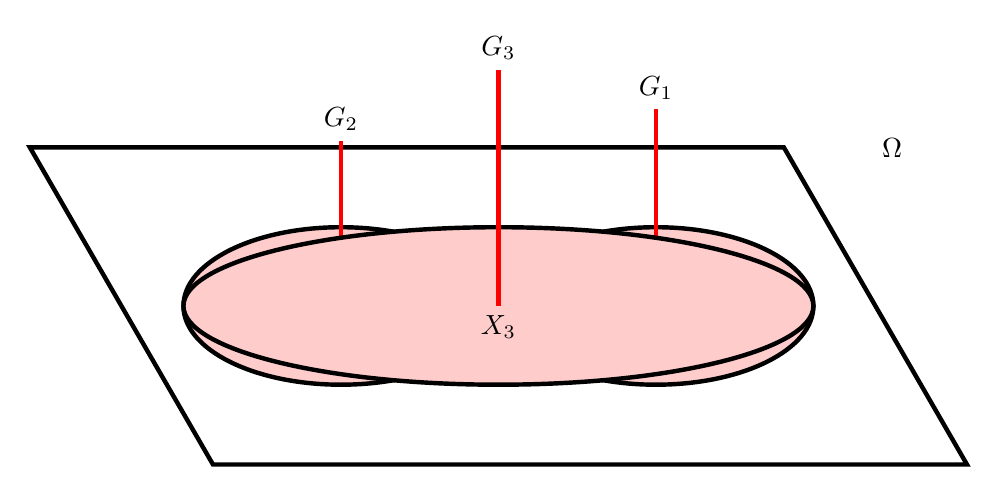
\begin{tikzpicture}
      \node at (5,2) {$\Omega$};

      \node[trap,ultra thick,trapezium stretches=false,minimum height=1cm,inner xsep=6pt]
      at (0,0) {};
      %% \path[draw,black,ultra thick] (0,0)--(11,0);
      \onslide<2>
      \draw[fill=red!20,ultra thick] (2,0) circle [x radius=2cm, y radius=1cm];
      \node[above] (p1) at (2,2.5) {$G_1$};
      \path[draw,red,ultra thick] (2,0) -- (p1);
      \node[below] at (2,0) {$X_1$};
      \onslide<3>
      \draw[fill=red!20,ultra thick] (-2,0) circle [x radius=2cm, y radius=1cm];
      \node[above] (p2) at (-2,2.1) {$G_2$};
      \path[draw,red,ultra thick] (-2,0) -- (p2);
      \node[below] at (-2,0) {$X_2$};
      \onslide<4>
      \draw[fill=red!20,ultra thick] (0,0) circle [x radius=4cm, y radius=1cm];
      \node[above] (p3) at (0,3.0) {$G_3$};
      \path[draw,red,ultra thick] (0,0) -- (p3);
      \node[below] at (0,0) {$X_3$};
      
      %% \tikz \draw (0,0) ellipse (2cm and 1cm);
      %% \tikz \draw (-1,0) ellipse (2cm and 1cm);
      %% \tikz \draw (2,0) ellipse (2cm and 1cm);
    \end{tikzpicture}
  \end{figure}
\end{frame}


%%       \draw[ultra thick] (0,0) circle [radius=3];
%%       \node at (3.2,0) {\Huge $\Omega$};
%%       \onslide<2>{
%%         \draw[red,ultra thick] (1.5,0) circle [radius=1.3] node {$X_1$};
%%       }
%%       \onslide<4>{
%%         \draw[green,ultra thick] (0.8,0.2) circle [radius=1.2] node {$X_2$};
%%       }

%% \begin{frame}
%% \begin{figure} 
%%   \centering
%%   \begin{tikzpicture}[scale=0.7]
%%       \path[draw,black,ultra thick] (0,0)--(11,0);
%%       \onslide<1-2>{
%%         \node[above] (p1) at (2,0.8) {$\phi(1)$};
%%         \path[draw,red,thick] (2,0) -- (p1);
%%         \node[below] at (2,0) {$1$};

%%         \node[above] (p2) at (4,4.2) {$\phi(2)$};
%%         \path[draw,red,thick] (4,0) -- (p2);
%%         \node[below] at (4,0) {$2$};

%%         \node[above] (p3) at (6,2.4) {$\phi(3)$};
%%         \path[draw,red,thick] (6,0) -- (p3);
%%         \node[below] at (6,0) {$3$};

%%         \node[above] (p4) at (8,1.0) {$\phi(4)$};
%%         \path[draw,red,thick] (8,0) -- (p4);
%%         \node[below] at (8,0) {$4$};

%%         \node[above] (p5) at (10,-2.0) {$\phi(5)$};
%%         \path[draw,red,thick] (10,0) -- (p5);
%%         \node[below] at (10,0) {$5$};
%%       }
%%       \onslide<2>{
%%         \node[above] at (2,5) {G(1)};
%%         \node[above] at (4,5) {G(2)};
%%         \node[above] at (6,5) {G(3)};
%%         \node[above] at (8,5) {G(4)};
%%         \node[above] at (10,5) {G(5)};
%%       }
%%       \onslide<3->{
%%         \node[above] (p1) at (2,-1.8) {$\phi(1)+G(1)$};
%%         \path[draw,red,thick] (2,0) -- (p1);
%%         \node[below] at (2,0) {$1$};

%%         \node[above] (p2) at (4,3.2) {$\phi(2)+G(2)$};
%%         \path[draw,red,thick] (4,0) -- (p2);
%%         \node[below] at (4,0) {$2$};

%%         \node[above] (p3) at (6,4.0) {$\phi(3)+G(3)$};
%%         \path[draw,red,thick] (6,0) -- (p3);
%%         \node[below] at (6,0) {$3$};

%%         \node[above] (p4) at (8,-2.0) {$\phi(4)+G(4)$};
%%         \path[draw,red,thick] (8,0) -- (p4);
%%         \node[below] at (8,0) {$4$};

%%         \node[above] (p5) at (10,2.0) {$\phi(5)+G(5)$};
%%         \path[draw,red,thick] (10,0) -- (p5);
%%         \node[below] at (10,0) {$5$};
%%       }
%%   \end{tikzpicture}

%%   \begin{center}
%%     \visible<2>{
%%      $G(i) \sim Gumbel(0)$ for  i=1..k\\
%%     }
%%     \visible<3>{
%%       Choose $x_j$ such that $j= argmax_i \{G(i) +\phi(i)\}$\\
%%     }
%%   \end{center}
%% \end{figure}  
%% \end{frame}

\end{document}
